% Paste these four standalone, caption-free figure environments into the paper.
% Compile from the repository root, or adjust the paths for your manuscript.
% Requires graphicx; the provided informs4 class already loads it.

% PFAOS: weak VI gap, n=25, 50, 100, 200, 500, 1000.
\begin{figure}[!htbp]
  \centering
  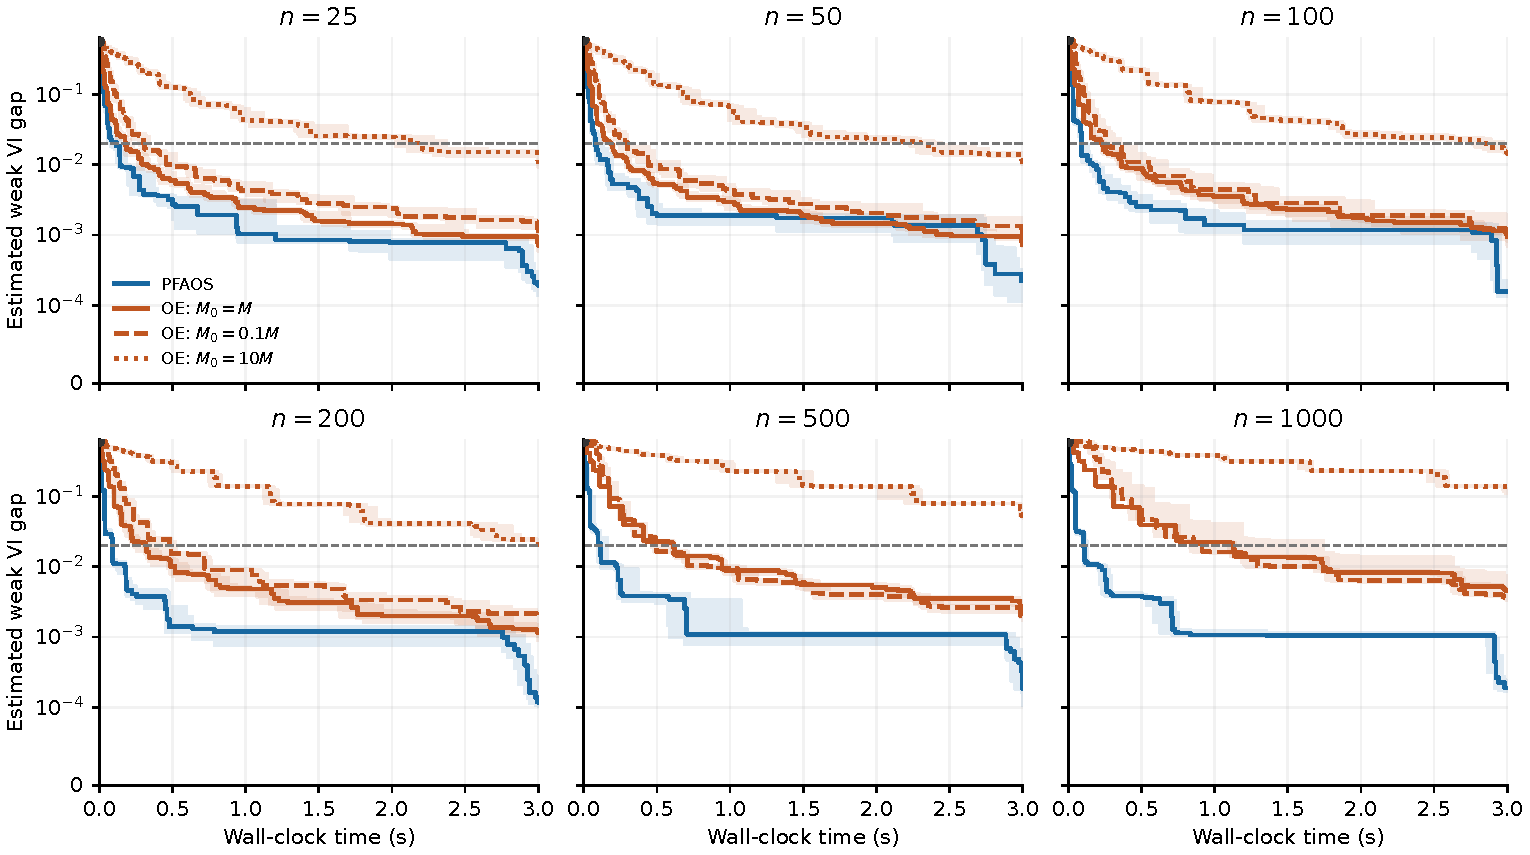
\includegraphics[width=0.97\linewidth]{results/figures/pfaos_residual.pdf}
\end{figure}

% PFAOS: constraint violation, zero for both methods at all six dimensions.
\begin{figure}[!htbp]
  \centering
  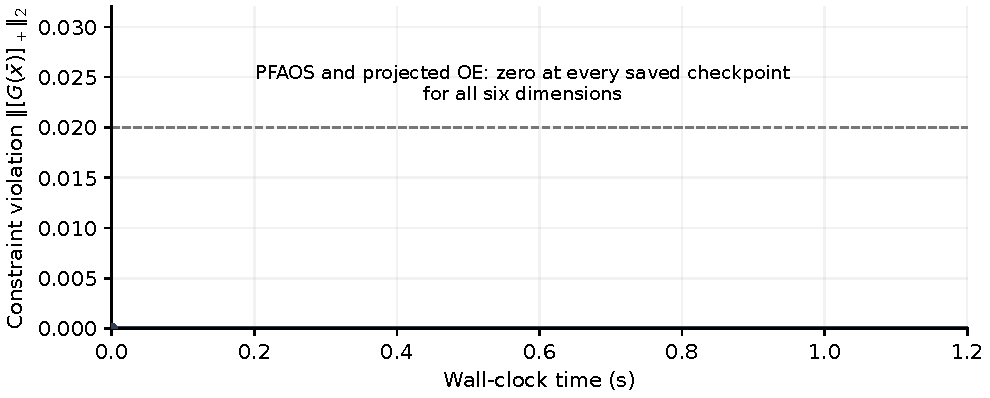
\includegraphics[width=0.92\linewidth]{results/figures/pfaos_violation.pdf}
\end{figure}

% MC-PFAOS: weak VI gap, n=50 and m=100.
\begin{figure}[!htbp]
  \centering
  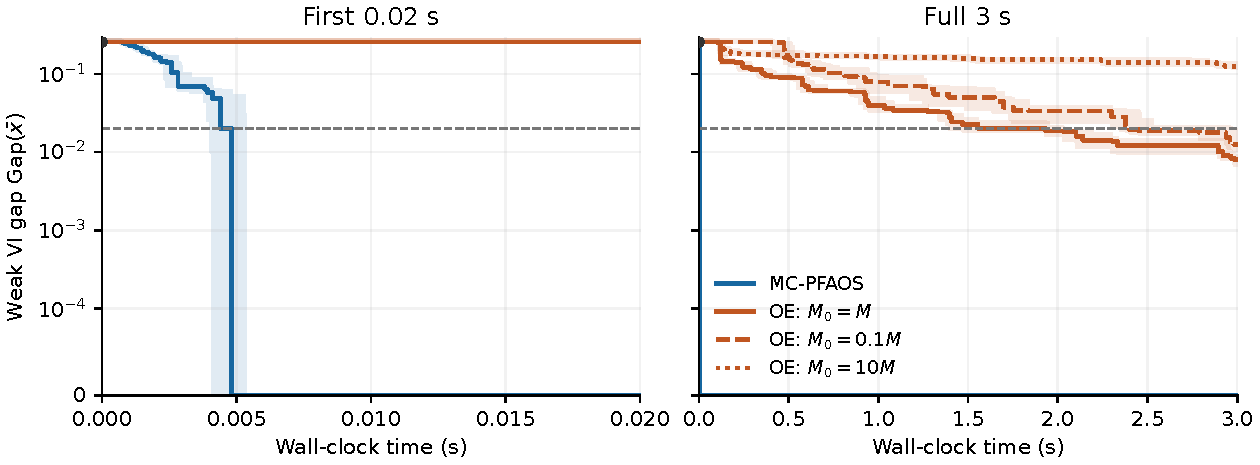
\includegraphics[width=0.92\linewidth]{results/figures/mc_residual.pdf}
\end{figure}

% MC-PFAOS: constraint violation, the same n and m.
\begin{figure}[!htbp]
  \centering
  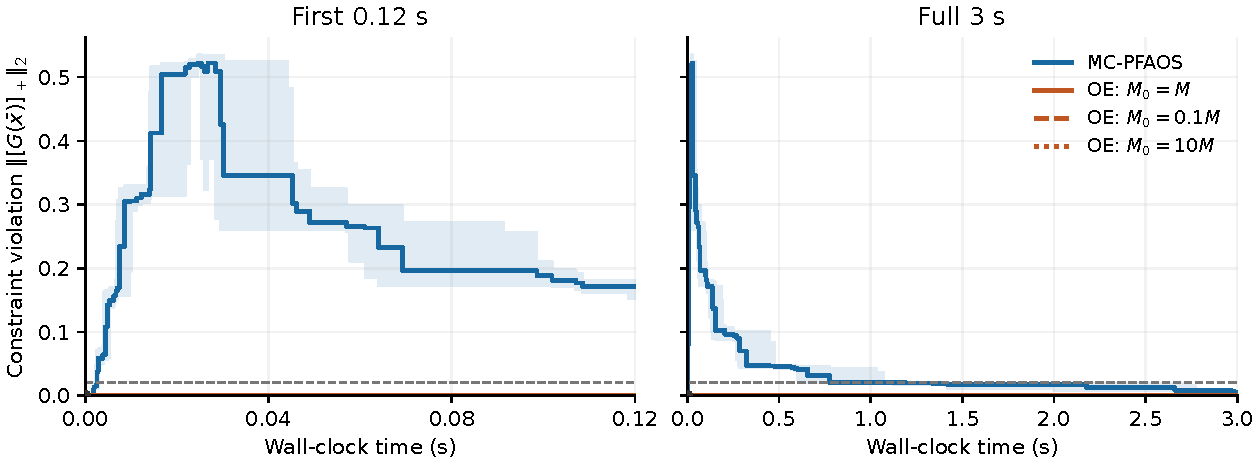
\includegraphics[width=0.92\linewidth]{results/figures/mc_violation.pdf}
\end{figure}
